\documentclass[uplatex,dvipdfmx]{jsarticle}

\usepackage[uplatex,deluxe]{otf} % UTF
\usepackage[noalphabet]{pxchfon} % must be after otf package
\usepackage{stix2} %欧文&数式フォント
\usepackage[fleqn,tbtags]{mathtools} % 数式関連 (w/ amsmath)
\usepackage{hira-stix} % ヒラギノフォント&STIX2 フォント代替定義(Warning回避)

\begin{document}

\title{タイトル}
\author{学生番号 氏名}
\date{2024年XX月XX日}
\maketitle
\section{はじめに}
こんな感じで文献引用する\cite{ref:nobukawa2023,ref:nobukawa2023_2}.

\subsection{社会的背景}
こんな感じで文献引用する\cite{ref:nobukawa2023,ref:nobukawa2023_2}.

\subsection{問題点}
%一般的な社会的背景を記述したパラグラフを複数配置, パラグラフの終わりは\parを入れる。
%最終パラグラフにはアイデアを記述する.

こんな感じで文献引用する\cite{ref:nobukawa2023,ref:nobukawa2023_2}.

\subsection{目的}
こんな感じで文献引用する\cite{ref:nobukawa2023,ref:nobukawa2023_2}.

\section{解決策としての提案手法}
%アイデアを実現する概要図を入れてその内容を説明する.
必要に合わせて,subsectionにわけて図を図\ref{fig:problem}や表\ref{table:presentation}
を引用しつつ説明する.

\begin{table}[h]
  \centering
  \caption{表のテンプレート}
  \label{table:presentation}
  \begin{tabular}{cl}
\hline
項目 & 内容 \\\hline \hline
1 & 社会的背景・問題点・主張 \\ \hline
2 & 解決策としての提案手法\\ \hline
3 & 提案手法の実現可能性の評価と妥当性の検証\\ \hline
  \end{tabular}  
\end{table}

\begin{figure}[h]
\centering
%\vspace{\baselineskip}
%\vspace{-1.5\baselineskip}
 \centering
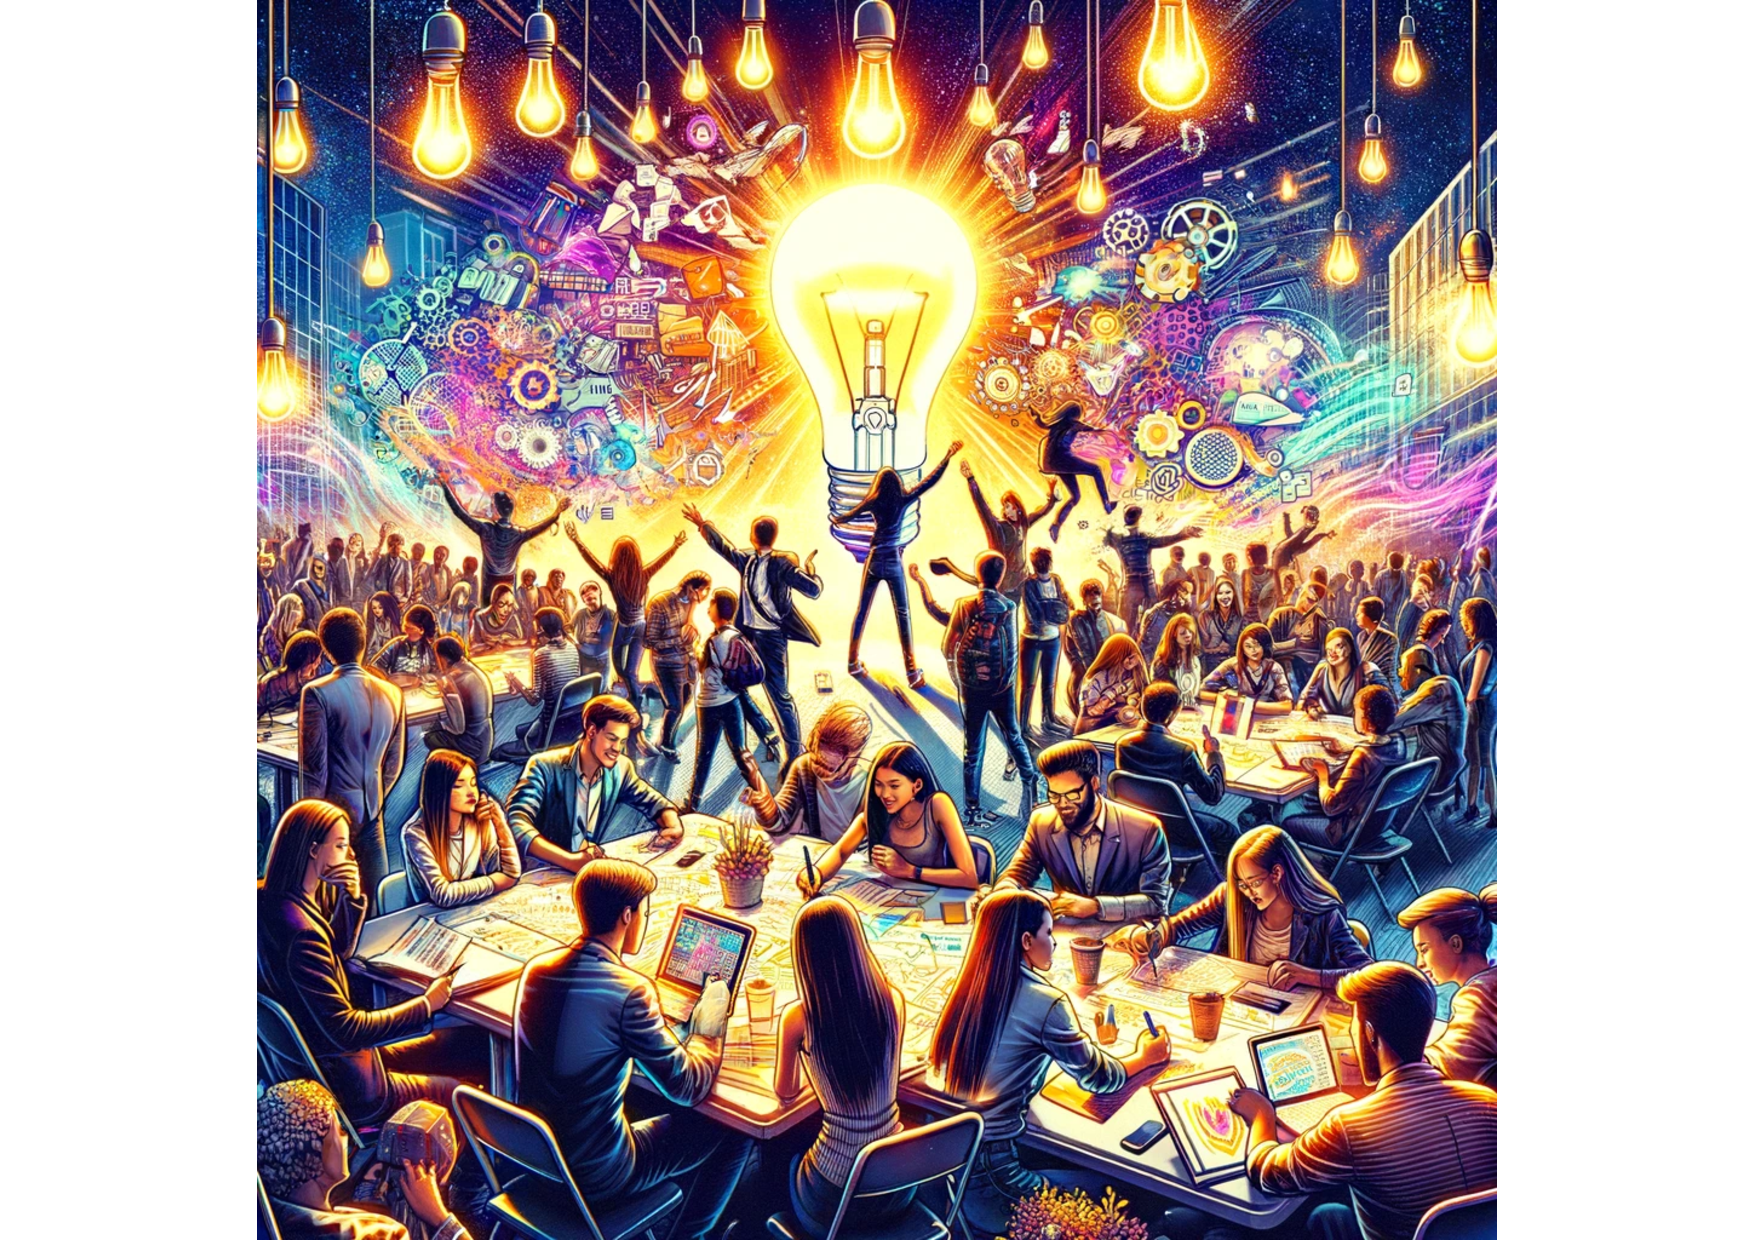
\includegraphics[width=10cm]{./Figs/idea.pdf}
%\vspace{\baselineskip}
%\vspace{-1.5\baselineskip}
\caption{図のテンプレート.}
%\vspace{-1.0\baselineskip}
\label{fig:problem}
\end{figure}


\section{提案手法の実現可能性の評価と妥当性の検証}
%

\section{おわりに}
%全体のまとめを簡潔に記述して,結論を述べる.




\begin{thebibliography}{9}
\bibitem{ref:nobukawa2023} 礒川悌次郎, \& 信川創. (2023). 脳・神経系における機能創発の解明を目指した数理モデリングとデータ駆動分析―局所神経回路から大域的全脳レベルまで―. 計測と制御, 62(10), 587-592.

\bibitem{ref:nobukawa2023_2}  信川創. "ヒトの認知行動を推定するアイマーカーの脳内メカニズム." 体育の科学, 73.10 (2023): 658-662.
\end{thebibliography}

\end{document} 
